\documentclass[runningheads]{llncs}
%
\usepackage[T1]{fontenc}
% T1 fonts will be used to generate the final print and online PDFs,
% so please use T1 fonts in your manuscript whenever possible.
% Other font encondings may result in incorrect characters.
%
\usepackage{graphicx}
\usepackage{float}
% Used for displaying figures. If possible, figure files should
% be included in EPS format.
%
% If you use the hyperref package, please uncomment the following two lines
% to display URLs in blue roman font according to Springer's eBook style:
%\usepackage{color}
%\renewcommand\UrlFont{\color{blue}\rmfamily}
\usepackage{hyperref}
\urlstyle{rm}
%
\begin{document}
%
\title{Designing Digital Twins for Progressive Fidelity: A Layered Architecture for Airport Operations Modelling with AI-Assisted Development}
%
\titlerunning{Digital Twins for Progressive Fidelity}
%
\author{Arthur Chevallier}
%
\authorrunning{A. Chevallier}
%
\institute{Luxembourg Institute of Science and Technology\\
\email{arthur.chevallier@list.lu}}
%
\maketitle              % typeset the header of the contribution
%
\begin{abstract}
Digital twins of complex cyber-physical systems are typically built as monolithic, closed-loop models that are difficult to extend and impossible to reproduce. We propose a layered fidelity architecture in which a digital twin begins as a pure event-driven simulation and progressively acquires physical, geospatial, and decisional capabilities---each phase building on the previous without architectural rewrites. We demonstrate this approach through Arthur International Airport (KART), a fully open-source airport digital twin implemented using a specification-first methodology with AI coding agent assistance. Structuring domain knowledge as machine-readable specification and skill files---readable by both human developers and large language model agents---is designed to reduce architectural errors and revision cycles. KART models flight operations, passenger flows, baggage handling, weather impacts, and incident cascades across nine microservices. All artefacts are publicly available.

\keywords{Digital twins \and Airport operations \and Cyber-physical systems \and AI-assisted software engineering \and Specification-driven development \and Simulation architecture \and Progressive fidelity.}
\end{abstract}
%
%
%
\section{Introduction}\label{sec:introduction}

Airports are canonical cyber-physical systems: aircraft, ground vehicles, passengers, baggage, and weather interact continuously under tight schedules and regulatory constraints. Digital twins---virtual counterparts that track a physical system through structured data flows~\cite{glaessgen2012,grieves2017}---are increasingly proposed as the operating paradigm for such infrastructure, yet in practice they are frequently delivered as monolithic, closed-loop models coupling simulation logic, geometry, live data feeds, and analytics in a single artefact. The difficulty is structural rather than incidental. Fidelity expectations grow over a project's lifetime: a team starts with logical operational modelling because it is cheap and testable, but stakeholders then demand physical realism, geospatial visualisation, live flight-tracking, and finally decision support. Each concern is individually well understood---network-level delay propagation has been modelled analytically~\cite{pyrgiotis2013}, and the cost of delay minutes has been quantified empirically~\cite{cook2009}---yet accreted onto a monolithic core, every step up in fidelity forces an architectural rewrite. Extensibility and reproducibility remain unresolved challenges~\cite{jones2020}: such a twin is hard to extend and effectively impossible to reproduce, its behaviour depending on live feeds, hidden local state, and undocumented assumptions.

We define digital twin in architectural terms: a graph-persisted representation of a system's entities and their relationships, kept synchronised with the source system's state through a fact-only event stream. Queries against the graph reflect current and historical state with bounded latency and support both monitoring and command issuance back into the source system. KART's ``source system'' is itself a synthetic simulation; the claim is that the pattern generalises to real physical systems. Read against the digital-model/shadow/twin taxonomy~\cite{kritzinger2018}, layers L0--L2 form a digital shadow, and only the decisional layer's approval-gated autonomous commands close the loop into a true digital twin.

The resulting design question is how a digital twin of a complex cyber-physical system should be architected so that fidelity can be acquired progressively without architectural rewrites, and whether specification-first development with AI coding agents can make such a system tractable for a single developer. Answering it requires three things: the layered architecture itself, the specification-and-skill methodology, and a complete end-to-end implementation whose costs, benefits, and failure modes can be examined honestly.

To answer these questions, we designed a four-layer fidelity architecture and instantiated it as Arthur International Airport (KART), a fully synthetic airport digital twin comprising roughly 45{,}000 lines of Python across nine microservices and roughly 28{,}000 lines of React/TypeScript dashboards. The system was developed by a single author over more than fifty sprints using a specification-first methodology: event-bus schemas, a graph data model, simulation rules, and one authoritative specification per service are written before implementation, complemented by ``skill files'' that encode reusable patterns and gotchas for both humans and LLM agents.

This paper makes four contributions:
\begin{enumerate}
  \item a layered fidelity architecture for digital twins in which each capability layer strictly consumes the contracts of the layer below, enabling progressive enrichment without re-platforming;
  \item a specification-first development methodology with skill files tailored to AI coding agents;
  \item KART, a fully open-source airport digital twin spanning flight operations, passenger flow, baggage handling, weather impacts, incident cascades, and financial planning;
  \item an honest account of lessons learned from fifty-plus sprints of agent-assisted development, including defects that slipped through review and the process changes that remediated them.
\end{enumerate}

The remainder of this paper is organised as follows. Section~\ref{sec:related} surveys related work on digital twins, airport simulation, and AI-assisted software engineering. Section~\ref{sec:architecture} presents the layered fidelity architecture. Section~\ref{sec:methodology} describes the specification-first development methodology and its integration with AI coding agents. Section~\ref{sec:implementation} details the KART implementation. Section~\ref{sec:evaluation} reports the evaluation approach and results, Section~\ref{sec:discussion} discusses findings and threats to validity, and Section~\ref{sec:conclusion} concludes.


\section{Related Work}\label{sec:related}

This section situates the paper against three bodies of work---digital-twin foundations, airport operations modelling, and AI-assisted software engineering---and states the gap it addresses.

The digital-twin concept originates in product-lifecycle management, where Grieves and Vickers articulated a virtual counterpart coupled to a physical asset through structured information flows~\cite{grieves2017}, and was subsequently formalised for NASA and US Air Force vehicles as a lifecycle-spanning computational representation~\cite{glaessgen2012}. For this paper's purposes the most consequential classification is Kritzinger et al.'s: digital models, shadows, and twins differ precisely in the degree of automated data flow between the physical and virtual sides---manual exchange, one-way automated flow, and closed two-way flow, respectively~\cite{kritzinger2018}. Characterisation studies confirm both the spread of the concept and the persistence of its problems. Jones et al.'s systematic review documents heterogeneous definitions and identifies extensibility and reproducibility among the unresolved engineering challenges~\cite{jones2020}, while Mohammadi and Taylor show the idea scaling from individual assets to city-scale human--infrastructure--technology systems observed in real time~\cite{mohammadi2017}. These accounts supply vocabulary and maturity levels, but none prescribes an architecture by which a deployed system ascends from shadow to twin without rework.

Airport operations research offers mature single-purpose models at both ends of the fidelity spectrum. At the analytical end, delay propagation through airport networks has been captured by queueing-plus-simulation models~\cite{pyrgiotis2013}, and the marginal cost of delay minutes has been quantified from airline operating data~\cite{cook2009}. At the predictive end, machine learning has been applied to boarding-time prediction~\cite{schultz2019}. Airport-specific digital twins are beginning to appear: an open-standards reference architecture validated for turnaround operations at Aberdeen International Airport~\cite{conde2022}, a simulation-based twin of landside operations~\cite{palasca2025}, and programme-level adoption guidance for airports~\cite{acrp2024}. Each delivers a single capability tier at fixed fidelity---deep analysis without live integration, or integrated visualisation without decision support---and none is designed so that further tiers can be accreted onto an existing core.

AI-assisted software engineering has meanwhile moved from demonstration to measurement. Codex established that large language models synthesise working programs from natural-language prompts~\cite{chen2021codex}; a controlled experiment measured substantially faster task completion with an LLM pair-programmer~\cite{peng2023copilot}; SWE-bench framed issue resolution on real repository defects as a benchmark~\cite{swebench2024}, with SWE-agent showing that agent-computer interfaces largely determine performance on it~\cite{yang2024sweagent}; and MetaGPT imposed standardised operating procedures on multi-agent software teams~\cite{hong2024metagpt}. What these evaluations capture, however, is local correctness---whether a generated patch passes its tests---not the architectural consistency of large multi-service systems assembled from many agent-authored parts. When an agent contributes code to one service of a distributed system, the failure surface extends beyond the patch itself: duplicated constants drift, event-field names diverge across producer and consumer, and recommendations that look correct in isolation are never wired into the bus. These inter-service coherence failures are precisely the defect class that specification-first discipline with machine-readable artefacts is designed to prevent, and they fall outside the scope of current benchmarks.

Beyond architectural questions, recent work has explored embedding machine-learning components directly into digital twins for predictive and prescriptive capability. Lightweight gradient-boosted models have been applied to passenger-flow forecasting at airport security checkpoints~\cite{ke2017,schultz2019}, and isolation-forest anomaly detectors have been deployed for operational-health monitoring in industrial digital twins~\cite{liu2008}. What the existing literature largely treats as standalone models, however, KART integrates as composable services behind a common event bus: the LightGBM forecaster, the Isolation Forest anomaly detector, the recommendation engine, and the Monte-Carlo scenario planner each consume the same operational graph and publish results as first-class events, making their outputs available to downstream consumers without tight coupling. This service-oriented integration mirrors the architectural principle that governs the simulation layers below, extending it into the decisional tier.

The gap, then, is not a missing component but a missing combination: no prior work couples a progressive-fidelity twin architecture with a specification-first methodology whose machine-readable artefacts are first-class inputs for LLM agents, instantiated end-to-end in an open-source airport digital twin. Section~\ref{sec:architecture} takes up the architectural half; Section~\ref{sec:methodology} the methodological one.

\section{Layered Fidelity Architecture}\label{sec:architecture}

This section answers (RQ1): what layered architecture allows a digital twin's fidelity to be acquired progressively? The answer is a stack of four capability layers---logical event-driven simulation, physical layout, geospatial and real-world data, and decision support---arranged so that each layer consumes only the contracts of the layer below. Fidelity is then acquired by accretion rather than rewrite: a project can begin at L0 and add capability over its lifetime without disturbing what already works. Against the digital-model/shadow/twin distinction from Section~\ref{sec:introduction}, layers L0--L2 constitute a digital shadow, and only the decisional layer closes the loop into a true twin.

The four layers are defined as follows.
\begin{itemize}
  \item \textbf{L0 --- logical event-driven simulation.} Domain state machines for flights, passengers, baggage, weather, and incidents communicate over a Kafka event bus~\cite{kreps2011} and persist entities in a Neo4j graph~\cite{angles2008}. No geometry, no external data: every quantity is logical, every interaction an event.
  \item \textbf{L1 --- physical layer.} Terminal layouts, gate positions, runway and taxiway geometry, together with the distances, walking times, and taxi times they induce.
  \item \textbf{L2 --- geospatial and real-world data layer.} Map-based visualisation (Mapbox/Cesium), ADS-B flight overlay, live and historical METAR weather, BTS schedule calibration, and OurAirports/OpenFlights reference data.
  \item \textbf{L3 --- decisional layer.} LightGBM queue forecasting~\cite{ke2017}, what-if and Monte-Carlo scenario analysis, discounted-cash-flow investment appraisal on Eurocontrol Standard Inputs~\cite{eurocontrol2024}, and autonomous operations whose commands reach the source system only through approval gates.
\end{itemize}

\begin{figure}[!ht]
\centering
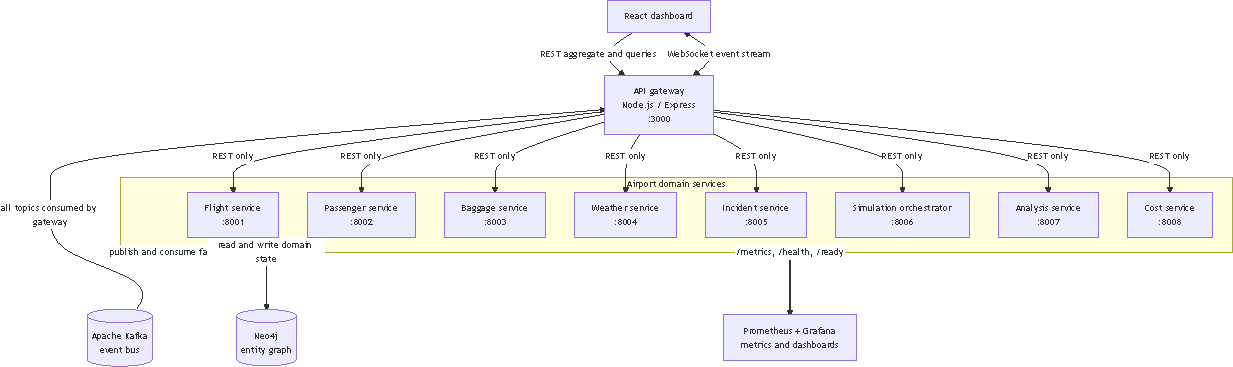
\includegraphics[width=\textwidth]{figures/arch.pdf}
\caption{KART system architecture. The gateway is the synchronous boundary for clients; Kafka decouples domain services, while Neo4j stores the operational graph.}
\label{fig:architecture}
\end{figure}

A set of architectural invariants keeps these layers composable. The simulation-clock contract forbids any service from reading wall-clock time: the orchestrator broadcasts ticks on a dedicated topic at configurable speed up to $3600\times$ real time, and all time-based logic reacts to ticks, enabling high-speed operation and deterministic replay. The event bus carries facts only: events record what happened, never what another service should do, so consumers remain independent of producers and the log doubles as an audit trail. Neo4j is the single source of truth for structural state: each service is the sole writer of its own node labels, and any in-memory cache is explicitly derived state, rebuildable from the graph after a restart. Every state change emits an event---there are no silent mutations---so the graph, dashboards, and analytical layers cannot drift apart.

\begin{figure}[!ht]
\centering
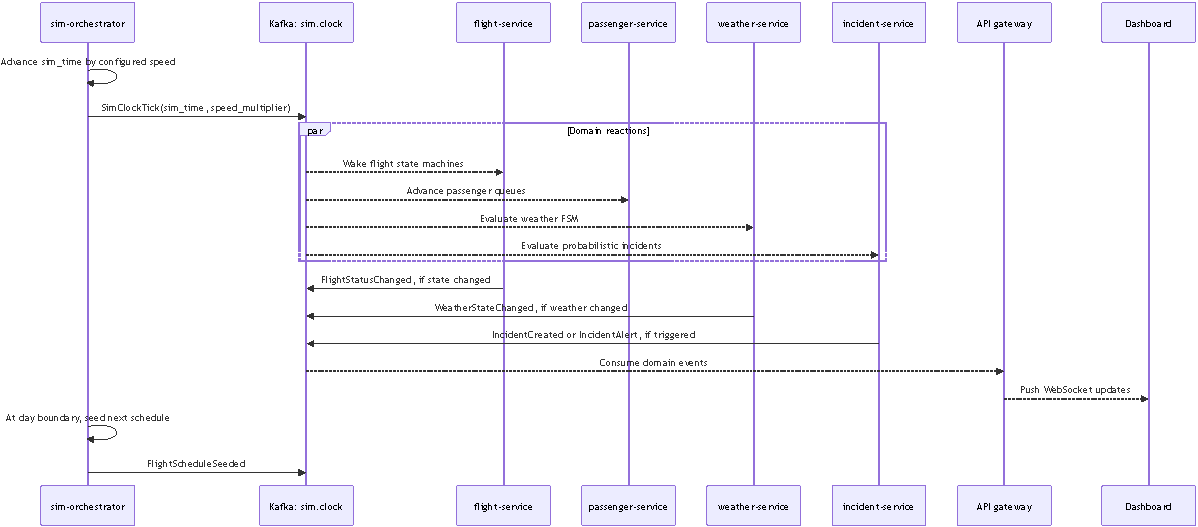
\includegraphics[width=\textwidth]{figures/clock.pdf}
\caption{Simulation-clock coordination. A single virtual-time stream drives every service, and resulting facts are pushed to the dashboard through the gateway.}
\label{fig:clock}
\end{figure}

Two further properties complete the design. Within each layer, capability deepens along a fixed ladder: visualisation $\rightarrow$ monitoring/alerting $\rightarrow$ prediction $\rightarrow$ prescription $\rightarrow$ actionability; a layer counts as mature when it has climbed this ladder, not merely when it renders something. Across layers, each layer consumes only the contracts of the layer below, and nothing above is visible from below, so upgrading a layer never breaks lower ones. The system's phased roadmap history---from pure simulation through map integration to forecasting and planning---landed without re-platforming; Section~\ref{sec:evaluation} returns to this evidence.

\section{Specification-First Development with AI Agent Integration}\label{sec:methodology}

This section answers (RQ2): how do machine-readable specifications and skill files affect the correctness and architectural consistency of implementations produced with LLM coding agents? The methodology rests on an inversion of the usual workflow: the specification is written first, is machine-readable, and is authoritative---implementation may not deviate from it, and where reality demands a change, the spec is updated first and the code follows. Before any service is implemented, four artefacts already exist: the event-bus schemas, the graph data model, the simulation rules, and one specification per service describing its endpoints, events, state machines, and ownership boundaries.

This discipline has an intellectual lineage older than language models: writing the authoritative description before the implementation echoes formal specification traditions~\cite{lamport2002}, and decomposing the system so that each service hides exactly one set of design decisions follows Parnas' information-hiding criteria~\cite{parnas1972}. What is new is the consumer. Human developers treat specifications as documentation that drifts from the code; an LLM agent treats them as ground truth to be followed literally. A stale spec once mildly misled human readers; now it actively misdirects the agent that writes the next change. Spec-first is therefore not ceremony but a correctness mechanism aimed at the entity that writes most of the code.

Complementing the per-service specifications are ``skill files'', which encode reusable project knowledge in a form readable by both humans and agents. Each skill file has three parts: concept explanation, copy-paste patterns, and gotchas. The patterns matter because code generation is imitation---an agent grounded in the project's idiomatic patterns produces consistent code, whereas one left to its prior defaults produces whatever its training data favoured. The gotchas encode failures that review caught the hard way and prevent their recurrence. Cross-cutting skills cover the FastAPI service skeleton, Neo4j/Cypher access, Kafka producers and consumers, the simulation clock and cascade rules, planning, and forecasting; each service additionally owns one skill file documenting its state machines and quirks.

Routing makes the difference between artefacts that exist and artefacts that get used. Agent entry points---\texttt{CLAUDE.md}, \texttt{AGENTS.md}, and editor rule files---instruct the agent to load the relevant specification and skill file before writing code, so authoritative context arrives by default. Hard rules function as guardrails against known LLM failure modes: no wall-clock time in business logic, no service-to-service HTTP calls, no silent mutations, and all data synthetic. Each maps one-to-one onto an architectural invariant from Section~\ref{sec:architecture}, so an agent violation is detectable by search or contract test rather than by luck.

The loop closes through sprint post-mortems: defects and near-misses found in review are promoted back into skill files as gotchas, making the same class of mistake unlikely twice. The knowledge base is thereby living, shared between human and machine readers, and accumulates detail where the project is most idiosyncratic.

\section{The KART Implementation}\label{sec:implementation}

KART instantiates the four-layer architecture of Section~\ref{sec:architecture} as a working system comprising roughly 45{,}000 lines of Python and roughly 28{,}000 lines of React/TypeScript dashboards. The stack is deliberately conventional---nine FastAPI domain services behind a thin Node.js/Express API gateway, a React/TypeScript dashboard suite, Kafka as the event backbone~\cite{kreps2011}, Neo4j as the graph store~\cite{angles2008}, Prometheus/Grafana/Loki/Jaeger for observability, and Kubernetes manifests with a staged CI pipeline---so that what the system tests is the architectural claim, not an exotic technology choice.

Domain depth is where the implementation earns the word ``twin''. The flight domain runs a nine-state lifecycle state machine with runway queueing and delay cascades that propagate up to five hops, mirroring network-level propagation models~\cite{pyrgiotis2013} (see Annex, Fig.~\ref{fig:flight-lifecycle}). Passenger flow models check-in, security congestion, and gate arrival, and feeds a LightGBM model that predicts security-queue depth ninety minutes ahead~\cite{ke2017,schultz2019}. Baggage travels a thirty-zone conveyor network with dangerous-goods screening. Weather is a four-state finite-state machine emitting ICAO-format METAR and TAF reports whose runway-capacity impacts feed directly into the flight domain (see Annex, Fig.~\ref{fig:weather-cascade}). A rule-based incident engine cascades five hazard types through the graph, spawning secondary incidents under explicit depth limits.

The digital twin is intentionally open at both its configuration and data boundaries. Airport identity, terminals, gates, runways, operational constants, and cascade limits are loaded from YAML rather than embedded in service logic; changing the airport therefore changes configuration, not event contracts or domain algorithms. A shared data-source registry exposes the same adapter interface to simulated, historical, and live providers, so new sources can be added without changing downstream consumers. This is the practical Open/Closed property of the twin: extend the represented world by adding configuration, fixtures, or adapters, while keeping the tested core closed to modification.

\begin{figure}[!ht]
\centering
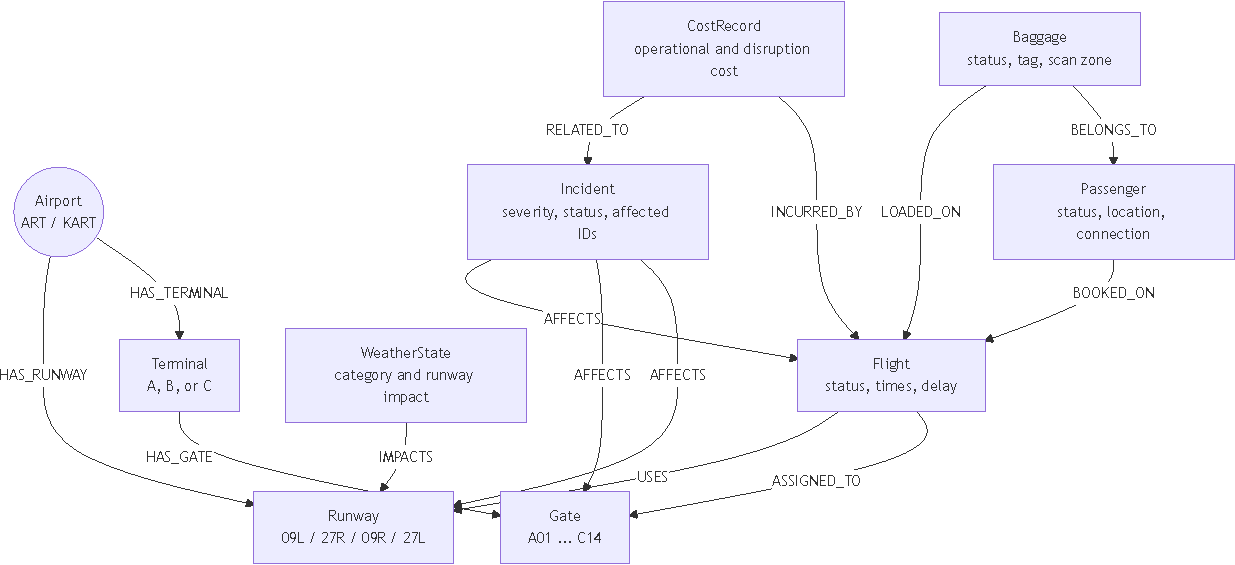
\includegraphics[width=\textwidth]{figures/graph.pdf}
\caption{Neo4j operational graph linking airport infrastructure, flights, passengers, baggage, weather, incidents, and cost records.}
\label{fig:graph}
\end{figure}

The simulated day is operationally plausible at scale: 420 flight movements, roughly 30{,}000 passengers, and roughly 36{,}000 baggage items, driven by a configurable simulation clock running up to $3600\times$ real time.

Crucially, the decisional layer is realised in production code rather than promised in the future tense. A financial service maintains profit-and-loss statements, passenger-rights liability under EC~261/2004~\cite{eu261}, and carbon accounting. A planning service runs Monte-Carlo infrastructure scenarios and NPV/IRR investment appraisals on Eurocontrol Standard Inputs~\cite{eurocontrol2024}. An analysis service provides anomaly detection~\cite{liu2008}, slot-allocation MILP, and an autonomous mode whose recommendations enter an approval queue and reach other domains only through per-domain command topics. This is the mechanism by which L3 closes the loop: commands are first-class, gated, and auditable, not advisory text on a dashboard.

The decisional layer comprises four integrated AI components. A LightGBM regression model forecasts security-queue depth across the three terminal checkpoints, trained on twelve contextual features including time-of-day, flight departure density, weather category, and incident status; the model retrains once per simulated hour and reports MAE at each cycle. An Isolation Forest detector monitors a fourteen-dimensional operational vector spanning queue depths, delay minutes, runway capacity, and vehicle utilisation, flagging anomalies with automated root-cause tracing through per-feature z-scores. A rule-based recommender generates up to three prioritised actions per tick across fourteen operation types---from opening security lanes to reassigning gates---routed through an approval queue that classifies each proposal as auto-executable, human-gated, safety-guarded, or operator-blocked. A Monte-Carlo scenario engine runs up to two hundred paired baseline-and-modified simulations to produce investment appraisals with NPV, IRR, and payback metrics grounded in Eurocontrol Standard Inputs~\cite{eurocontrol2024}.

Reproducibility, finally, is structural rather than aspirational. All specifications, skill files, infrastructure definitions, and data pipelines are open source at \url{https://github.com/Jupiter41/arthur-airport} (DOI: 10.5281/zenodo.22065741), and the airport's identity lives in configuration rather than code---a different airport is a YAML file, not a fork.

\section{Evaluation}\label{sec:evaluation}

This section answers (RQ3): what does a complete end-to-end implementation reveal about the costs, benefits, and failure modes of the approach? The method is a qualitative case study of a single-developer project across fifty-plus sprints, following established software-engineering case-study guidelines~\cite{runeson2009} and using the repository's documented revision history as the evidence trail. The setting trades breadth of generalisation for longitudinal depth: every design decision, defect, and remediation in the project's life is reconstructable from the record.

Engineering quality is measured by the test and integration apparatus. The system carries 946 test functions (counted as \texttt{def test\_*} definitions across \texttt{tests/unit/} and \texttt{tests/integration/}; parametrised fixtures expand the collected case count), including event-chain contract tests that verify cross-service behaviour and consumer idempotency tests that verify safe replays. These are executed by a staged CI pipeline: lint, unit, integration, Docker build, end-to-end smoke, and load tests. The staging matters as much as the counts---each stage isolates a distinct failure class, so an agent-introduced regression surfaces with a diagnosis attached rather than as a mysterious integration failure.

At the project's close, the operational graph links 13 entity types across 14 Kafka topics and 171 domain API endpoints (those exposed through the API gateway, excluding internal inter-service routes), governed by 9 service specifications and 15 skill files. The test suite grew from 256 at Sprint 10 to 946 at the project's close---a 3.7× increase that tracked the codebase's expanding scope without requiring architectural rewrites.

Functional demonstrations exercise the layers together rather than in isolation. The flagship walkthrough traces one causal chain end to end: weather degradation cuts runway capacity, which lengthens the departure queue, which produces gate conflicts, which break passenger connections, which materialise as quantified EC~261 exposure in the financial layer. Counterfactual replay re-runs past operational decisions under altered conditions, and a Monte-Carlo investment scenario compares baseline against expanded infrastructure in NPV terms---demonstrations spanning L0 through L3 within a single system.

The methodology evidence bears directly on RQ2. Qualitative evidence from the mid-project architectural audit (Section~\ref{sec:discussion}) surfaced three distinct classes of defect---diverging duplicated constants, dashboard recommendations that were never executed, and ML endpoints reporting success without training---none caught by the existing test suite. Their common cause was implementation drifting silently away from its governing specification. The remedy adopted was single-source-of-truth tests that lock constants and schemas against drift between services, directly extending the specification-first mechanism from Section~\ref{sec:methodology}. That these defect classes required a dedicated audit to surface suggests that spec-first discipline narrows, but does not by itself close, the gap between what a service is specified to do and what agent-authored code actually does.

The scope is stated plainly: no controlled human study, all data synthetic by design, and quantitative claims limited to system-level engineering metrics. Section~\ref{sec:discussion} treats these limits as threats to validity in full.

\section{Discussion}\label{sec:discussion}

Four practices proved to compound rather than merely add up. Contract-first discipline kept services independently understandable and testable. Config-driven airport identity applied the Open/Closed principle at the level of the whole system. Promoting duplicated Kafka transport code into a shared library removed an entire class of copy-paste divergence, and hexagonal refactors moved domain logic behind ports so that it could be unit-tested without containers. None of these was expensive at adoption; each paid for itself repeatedly afterwards.

The project's most instructive episode was an iteration on its own base. A mid-project architectural audit surfaced defects characteristic of fast agent-assisted development: constants diverging between copies of duplicated code, recommendations displayed on dashboards but never executed, and ML endpoints reporting success without having trained a model. Every one was remediated through the same specification-first process that produced the system in the first place.

The cautionary finding is how easily such defects slip through. Without systematic review they pass unnoticed, and several reached user-facing dashboards before detection. Audit-style and mutation-style test guards~\cite{demillo1978} are therefore a first-class part of the workflow, not an afterthought appended after a bad sprint.

A specification only constrains what an agent is told to do; it cannot guarantee what the agent actually writes. Even with an authoritative spec, an LLM agent can produce code that superficially conforms while silently drifting from it---a hallucinated adapter, a copied constant that no longer matches its source of truth, an endpoint that returns a plausible response without doing the work it claims. Spec-first discipline lowers the rate of this drift; it does not eliminate it, because the spec constrains intent, not execution. The practical consequence is that spec-versus-implementation conformance has to be checked periodically as a standing practice, rather than assumed from the existence of a good specification.

Underlying the specific practices is a trustworthiness principle: delete or make real anything that advertises capability it lacks. A recommendation that is never executed is decoration; an endpoint that reports success without training is fiction. Predicted-versus-actual outcome measurement closes the loop, so the system's claims about itself are continuously checked against what actually happens.

The approach generalises beyond airports. The layered-fidelity template applies wherever a cyber-physical domain has tiers of capability that arrive over a project's lifetime---ports, hospitals, and warehouses are immediate candidates. The spec-plus-skill methodology applies wherever LLM agents write substantial code. Digital twins have already scaled from individual products to entire cities~\cite{mohammadi2017}. The piece this paper adds is an acquisition path that does not demand re-platforming at each step.

Finally, threats to validity. The study has a single developer, a single domain, self-reported revision-cycle claims, and synthetic ground truth---the standard limits of the single-case method~\cite{runeson2009}. Moreover, because the same developer accumulated domain knowledge over the project's lifetime, the observed reduction in defect rates across sprints cannot be cleanly separated from learning effects; the spec-first methodology and growing domain expertise are confounded in this single-case study. The claims defended here are narrow: that the architecture is sound and the methodology reproducible. Measured productivity effects are not claimed to generalise unchanged to other teams.

\section{Conclusion}\label{sec:conclusion}

This paper asked three questions. How should a digital twin of a complex cyber-physical system be architected so that fidelity can be acquired progressively? Does specification-first development with AI coding agents make such a system tractable for a single developer? And what does a complete implementation reveal about the approach's costs and failure modes? The answers: (RQ1) a four-layer architecture with strict upward-only dependencies supports progressive fidelity without rewrites; (RQ2) machine-readable specifications and skill files steer LLM agents toward architecturally consistent implementations; and (RQ3) the complete implementation confirms feasibility while exposing the review practices---audit guards, contract tests, post-mortem feedback into skill files---needed to keep agent-generated systems trustworthy.

The broader claim is that progressive fidelity plus specification-first agent development makes airport-scale digital twins tractable for a single developer. Neither half suffices alone: layering without executable process knowledge produces drift, and process knowledge without a stable architecture produces rewrites. KART demonstrates the combination across fifty-plus sprints, and every artefact---specifications, skill files, infrastructure, and code---is open.

What the case study also makes visible is where human judgement sits once an agent writes most of the code. Agent-assisted development did not remove the engineer from the architecture; it relocated their contribution upstream, from writing individual services to fixing the domain's boundaries and its direction of growth before any service existed. Specification-first development, in this sense, is as much about a human author committing early to a domain's scope and its maturity path as it is about constraining what an agent may build.

Future work follows the gaps. Command-topic coverage must be completed across all domains, so that every decisional capability can act and not only advise. The twin's deterministic clock and persistent event log make it a natural benchmark environment for multi-agent reinforcement learning, a setting current benchmarks lack. And because an airport is now a configuration file rather than a codebase, multi-airport network studies---delay propagation across federated twins---are within reach of the same single-developer methodology.

\section*{Acknowledgments}

This research received no specific grant from any funding agency in the public, commercial, or not-for-profit sectors. The author thanks colleagues at the Luxembourg Institute of Science and Technology for their review of and feedback on earlier drafts of this manuscript. All computation, development, and infrastructure for the KART implementation were carried out on the author's own resources, without external infrastructure support.

\section*{Use of AI}

Artificial intelligence tools were used to support the writing and editing of this manuscript. These tools helped with text rephrasing, proofreading, and improving clarity, but all scientific content, interpretations, and conclusions were produced and validated by the authors. No generative AI system was used to create data, analyses, or results. The authors take full responsibility for the accuracy and integrity of all statements in the paper.

\newpage
\section*{Annex}

\begin{figure}[H]
\centering
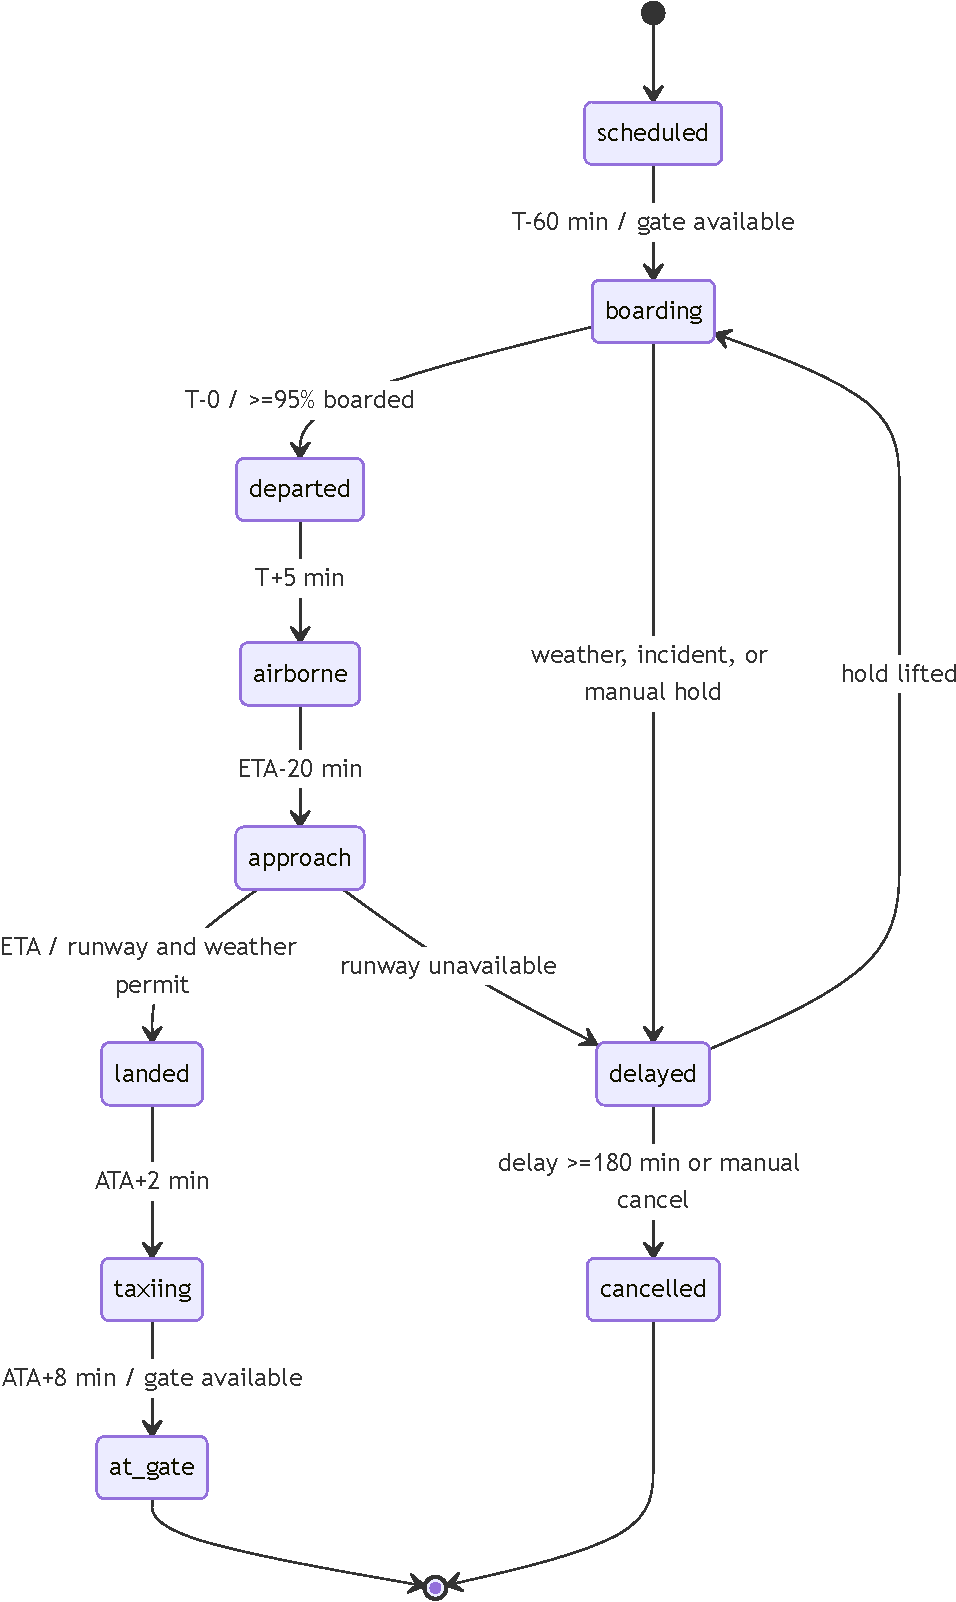
\includegraphics[width=\textwidth]{figures/flight-lifecycle.pdf}
\caption{Flight lifecycle driven by simulated time and constrained by gates, runways, weather, incidents, and boarding progress.}
\label{fig:flight-lifecycle}
\end{figure}

\begin{figure}[H]
\centering
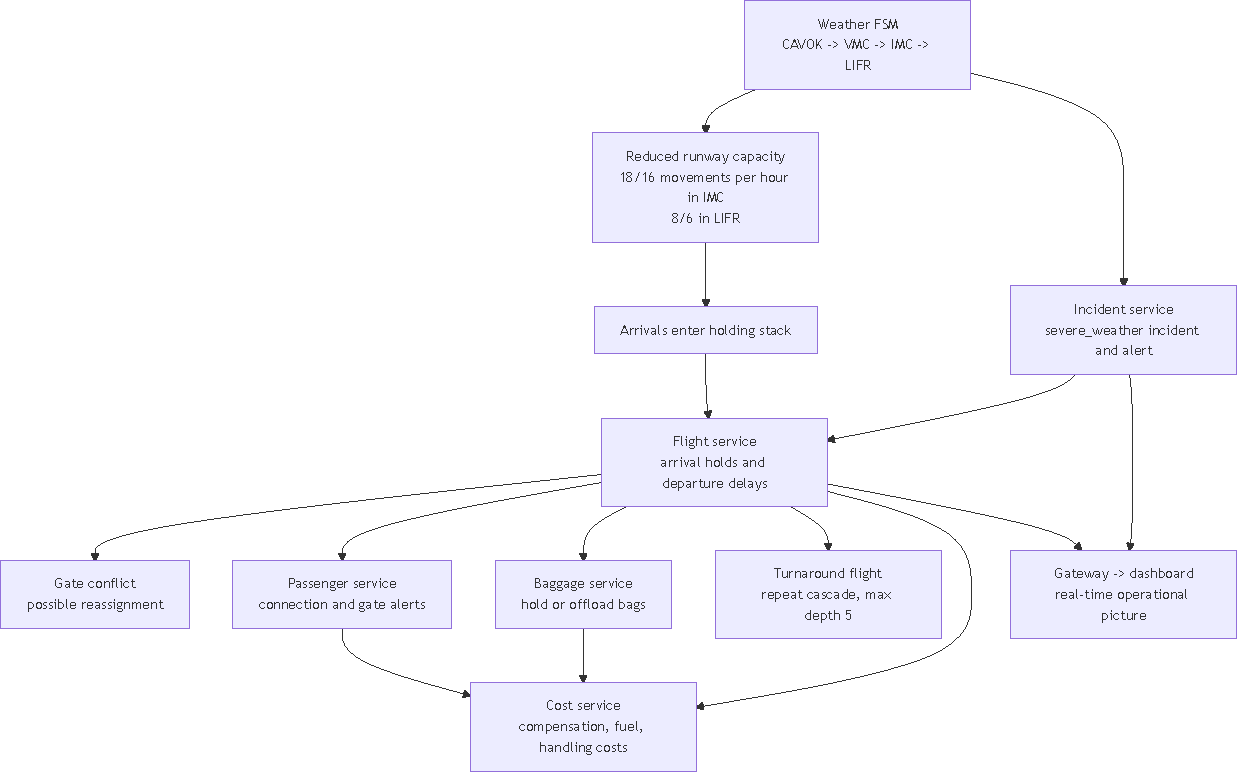
\includegraphics[width=\textwidth]{figures/weather-cascade.pdf}
\caption{Causal propagation from weather degradation to runway capacity, flight delays, passenger and baggage disruption, and operational cost.}
\label{fig:weather-cascade}
\end{figure}

\newpage
%
% ---- Bibliography ----
%
\bibliographystyle{splncs04}
\bibliography{refs.bib}

\end{document}
